\begin{figure}[H]
    \centering
    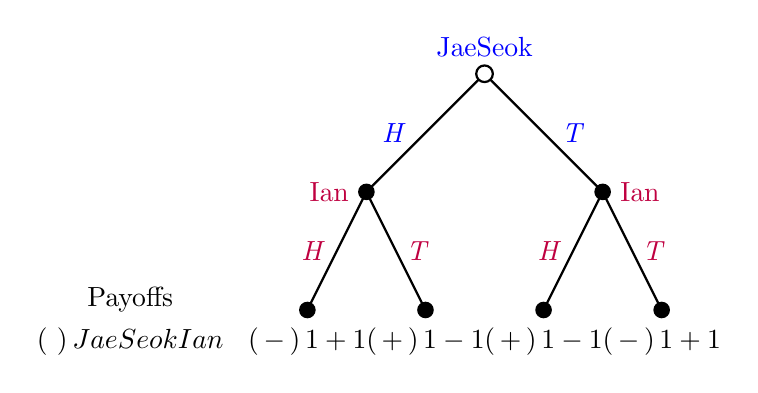
\begin{tikzpicture}[scale=1.5]
        % First mover's move
        \draw[thick] (0,0) -- (-1,-1) node[pos=.5,left=0.1cm] {\color{blue}\textit{H}};
        \draw[thick] (0,0) -- (1,-1) node[pos=.5,right=0.1cm] {\color{blue}\textit{T}};
        % Second mover's move
        \draw[thick] (-1,-1) -- (-1.5,-2) node[pos=.5,left] {\color{purple}\textit{H}};
        \draw[thick] (-1,-1) -- (-0.5,-2) node[pos=.5,right] {\color{purple}\textit{T}};
        \draw[thick] (1,-1) -- (0.5,-2) node[pos=.5,left] {\color{purple}\textit{H}};
        \draw[thick] (1,-1) -- (1.5,-2) node[pos=.5,right] {\color{purple}\textit{T}};
        % Nodes
        \draw[fill=white, thick] (0,0) circle[radius=2pt];
        \node[above=0.1cm] at (0,0) {\color{blue}JaeSeok};
        \fill (1,-1) circle (2pt) node[right=0.1cm] {\color{purple}Ian};
        \fill (-1,-1) circle (2pt) node[left=0.1cm] {\color{purple}Ian};
        % Payoffs
        \fill (-1.5,-2) circle (2pt) node[below=0.1cm] {$\begin{pmatrix} -1 \\ +1 \end{pmatrix}$};
        \fill (-0.5,-2) circle (2pt) node[below=0.1cm] {$\begin{pmatrix} +1 \\ -1 \end{pmatrix}$};
        \fill (0.5,-2) circle (2pt) node[below=0.1cm] {$\begin{pmatrix} +1 \\ -1 \end{pmatrix}$};
        \fill (1.5,-2) circle (2pt) node[below=0.1cm] {$\begin{pmatrix} -1 \\ +1 \end{pmatrix}$};
        \node[above] at (-3,-2.1) {Payoffs};
        \node[below=0.1cm] at (-3,-2) {$\begin{pmatrix} \text{JaeSeok} \\ \text{Ian} \end{pmatrix}$};
    \end{tikzpicture}
\end{subfigure}